\newpage
\section{Auswertung}

% -------------Magnetfeld------------
\subsection{Magnetfeldmessung}
Zu Beginn des Experiments wird das Magnetfeld in Abhängigkeit des Spulenstroms bestimmt (\ref{tab:Br}).
Zwischen den beiden Größen besteht ein linearer Zusammenhang, daher lässt sich die Kurve durch eine Ausgleichsgerade annähern.
% Data 2
\begin{table}[H]
    \centering
    \begin{tabular}{c c}
        \toprule
        $I_{Spule} \;/\;$A & $B\;/\;$mT\\
        \midrule
        0,0                 &0,0\\
        0,5                 &132,4\\
        1,0                 &270,0\\
        1,5                 &413,7\\
        2,0                 &556,4\\  
        2,5                 &698,3\\
        3,0                 &828,3\\
        3,5                 &956,0\\
        4,0                 &1063,9\\
        4,5                 &1145,2\\
        5,0                 &1204,5\\
        \bottomrule
    \end{tabular}
    \caption{Magnetfeldmessung (reihe)}
    \label{tab:Br}
\end{table}
% Plot 2
\begin{figure}[H]
    \centering
    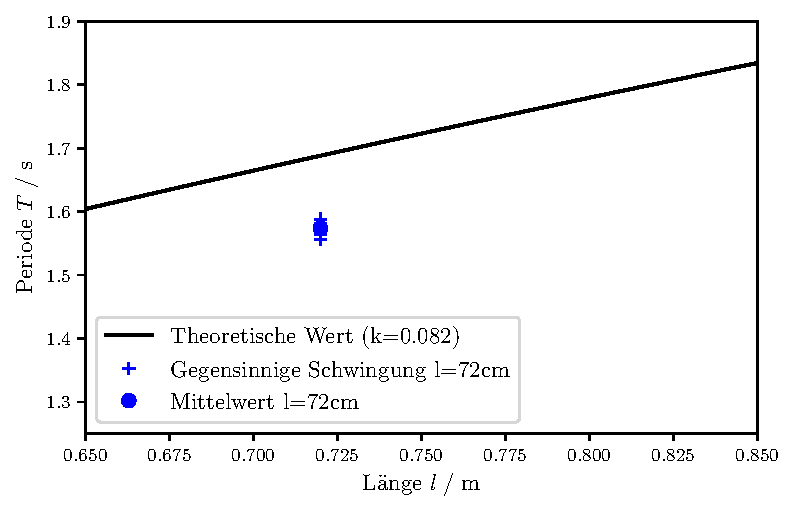
\includegraphics{build/plot2.pdf}
    \caption{B-Feld Messung}
    \label{fig:Br}
\end{figure}
Mit der Ausgleichsgeraden
\begin{align*}
    y &= mx + b\\
    m &= \SI{251\pm 8}{\milli \tesla \per \ampere} \\  
    b &= \SI{32\pm 24}{\milli \tesla}\\
\end{align*}
Aus der Umkerfunktion dieser Ausgleichsrechnung lässt sich in den folgenden Berechnungen das B-Feld aus dem angelegten Spulenstrom bestimmen.

\subsection{Die Bestimmung der mikroskopischen Parameter}
Über die gemessene Hall Spannung,das dazugehörige B-Feld und den Querstrom kann man über \ref{eqn:U_Hall} auf die Anzahl der Ladungsträger pro Volumen schließen.
\begin{equation*}
    n = -\frac{1}{e_0 U_H}\cdot \frac{B\cdot I_q}{d}
\end{equation*}
Weiterhin lässt sich mit den so errechneten Werten für n der Energie Parameter $E_F$ berechnen.
\begin{equation*}
    E_F = \frac{h^2}{2 m_0}\cdot \left(\frac{3}{8\pi}\cdot n \right)^{\frac{2}{3}}
\end{equation*}
Über $E_F$ lässt sich der nächste Parameter, die Totalgeschwindigkeit $|\bar{v}|$, berechnen.
\begin{equation*}
    |\bar{v}| = \left(\frac{2 E_F}{m_0}\right)^{\frac{1}{2}}
\end{equation*}
Außerdem lässt sich aus n und der zuvor berechneten spezifischen Leitfähigkeit $\rho$ die mittlere Flugzeit $\bar{\tau}$ berechnen.
\begin{equation*}
    \bar{\tau} = 2 \frac{m_0}{e_0^2} \cdot \frac{1}{n \rho}
\end{equation*}
Aus der mitlleren Flugzeit $\bar{\tau}$ kann dann noch die mittlere freie Weglänge $\bar{l}$ bestimmt werden.
\begin{equation*}
    \bar{l} = \bar{\tau} \cdot |\bar{v}|
\end{equation*}
Nun muss noch die Beweglichkeit der Ladungsträger $\mu$ über das äußere elektrische Feld $\vec{E}$ und die Driftgeschwindigkeit $\vec{\bar{v}}_d$ bestimmt werdenbestimmt werden
\begin{align*}
    \vec{\bar{v}}_d &= -\frac{n \cdot e_0}{j} \\
    \Delta \vec{\bar{v}} &= 2\cdot \vec{\bar{v}}_d\\
    \mu = \frac{E}{\vec{\bar{v}}_d} &= - \frac{\Delta \vec{\bar{v}}\cdot m_0 }{\vec{\bar{v}}_d \cdot \bar{\tau} \cdot e_0}\\
\end{align*}

%|||||||||||||||||||||||||||||||||||||||||||||||||||||||||||||||||||||||||||||||||||||||||||||||||||||||||||||||||


% --------KUPFER
\subsection{Kupfer}
\subsubsection{Geometrische Messungen und Wiederstand}
Die Dicke des Kupferblatts konnte auf der Apparatur abgelesen werden.
Die Länge des Kupferdrahts konnte auch abgelesen werden, der Wiederstand wurde jedoch gemessen.
\begin{align*}
    d_{Cu} &= \SI{18}{\micro \meter} \\
    l_{Cu} &= \SI{137}{\centi \meter}\\
    R_{Cu} &= \SI{2,734}{\ohm}\\
    r_{Cu} &= \frac{1}{2}\cdot \SI{0,218}{\milli \meter}
\end{align*}
Daraus lässt sich die spezifische Leitfähigkeit des Materials berechnen.
\begin{align*}
    \rho_{Cu} &= R_{Cu}\cdot \frac{\pi r_{Cu}^2}{l_{Cu}}\\
    \rho_{Cu} &= \SI{0,074\pm0,007}{\micro \ohm \meter}\\
    \rho_{Cu,literatur} &= \SI{0,018}{\micro \ohm \meter} %https://oerttel.net/data/documents/Leitfaehigkeit.pdf
\end{align*}
\subsubsection{Hall Spannung bei konstantem B-Feld}
Um die Abhängigkeit der Hall Spannung vom anliegenden Querstrom $I_q$ festzustellen wurde der Spulenstrom $I_B$ konstant auf 5 Ampere gehalten.
% Data 4
\begin{table}[H]
    \centering
    \begin{tabular}{c c c}
        \toprule
        $I_B \;/\;$A & $U_H\;/\;$mV & $I_q \;/\;$A\\
        \midrule
            5                   & 0,0029&             0\\
            5                   & 0,0005&             1\\
            5                   &-0,0015&             2\\
            5                   &-0,0030&             3\\
            5                   &-0,0044&             4\\
            5                   &-0,0056&             5\\
            5                   &-0,0075&             6\\
            5                   &-0,0088&             7\\
            5                   &-0,0110&             8\\
            5                   &-0,0129&             9\\
            5                   &-0,0140&             10\\
        \bottomrule
    \end{tabular}
    \caption{Hall Spannung für Kupfer- konstantes Magnetfeld}
    \label{tab:Cu_I}
\end{table}
% Plot 4
\begin{figure}[H]
    \centering
    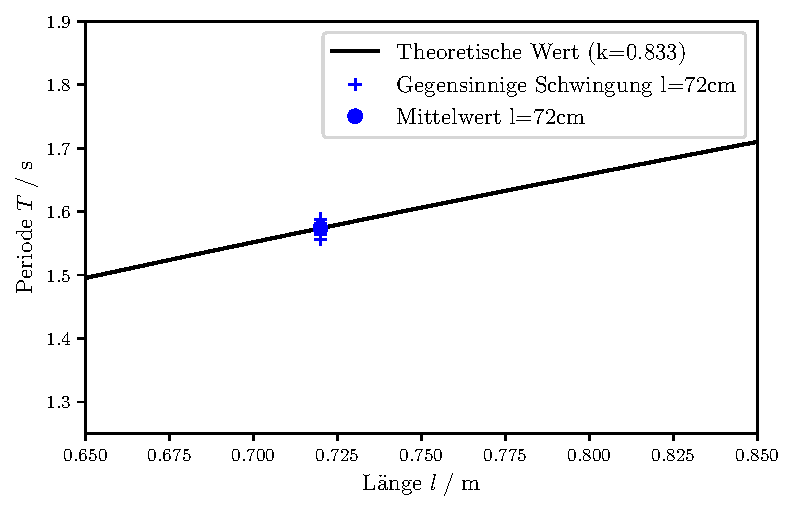
\includegraphics{build/plot4.pdf}
    \caption{Hall Spannung in Abhängigkeit vom Querstrom - Kupfer}
    \label{fig:Cu_I}
\end{figure}
Mit der Ausgleichsgeraden
\begin{align*}
    y &= mx + b\\
    m &= -0.001654\pm 0.00004\\  
    b &=  0.0023\pm 0.0003\\
\end{align*}

\subsubsection{Hall Spannung bei konstantem Querstrom}
Um die Abhängigkeit der Hall Spannung vom äußeren Magnetfeld $B$ festzustellen wurde der Querstrom $I_q$ konstant auf 10 Ampere gehalten.
% Data 3
\begin{table}
    \centering
    \begin{tabular}{c c c}
        \toprule
        $I_{B} \;/\;$A & $U_H\;/\;$mV & $I_{q} \;/\;$A\\
        \midrule
        0                   &0,0081              &10\\
        0,5                 &0,0055              &10\\
        1,0                 &0,0039              &10\\
        1,5                 &0,0012              &10\\
        2,0                 &-0,0008             &10\\
        2,5                 &-0,0025             &10\\
        3,0                 &-0,0048             &10\\
        3,5                 &-0,0068             &10\\
        4,0                 &-0,0086             &10\\
        4,5                 &-0,0097             &10\\
        5,0                 &-0,0110             &10\\
        \bottomrule
    \end{tabular}
    \caption{Hall Spannung für Kupfer- konstanter Duchflussstrom}
    \label{tab:Cu_B}
\end{table}
% Plot 3
\begin{figure}[H]
    \centering
    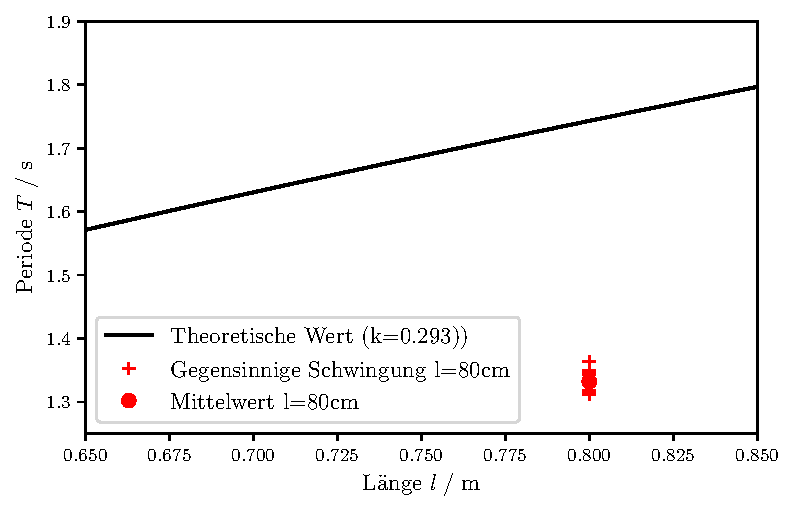
\includegraphics{build/plot3.pdf}
    \caption{Hall Spannung in Abhängigkeit vom Magnetfeld - Kupfer}
    \label{fig:Cu_B}
\end{figure}
Mit der Ausgleichsgeraden
\begin{align*}
    y &= a \cdot x + b\\
    a &=  \SI{-15,4 \pm 0,5 }{\square \meter \per \second}\\
    b &=  \SI{7,9\pm0,4}{\tesla}\\
\end{align*}
Daraus ergibt sich n mit:
\begin{align}
    n = \SI{2,24\pm0,06 e29}{\per \cubic \metre}
\end{align}

\subsubsection{Werte für die mikroskopischen Parameter}
%----------Tabelle
\begin{table}
    \centering
    \begin{tabular}{c c c c c}
        \toprule
        $U_H$ & $B$ & $n$  & $\bar{\tau}$ & $\vec{\bar{v}}_d$ \\
        \midrule
        $0.00740\pm 0.00034  $& $33\pm 24                 $& $(4.8\pm 3.4)\cdot 10^{21}      $& $(2.0\pm 1.4)\cdot 10^{-7}      $& $(8\pm 5)\cdot 10^{2}          $\\
        $0.00546\pm 0.00035  $& $159\pm 24                $& $(1.93\pm 0.33)\cdot 10^{22}    $& $(4.9\pm 1.0)\cdot 10^{-8}      $& $(3.1\pm 0.5)\cdot 10^{3}      $\\
        $0.0035\pm 0.0004    $& $284\pm 25                $& $(2.1\pm 0.6)\cdot 10^{22}      $& $(4.6\pm 1.4)\cdot 10^{-8}      $& $(3.3\pm 0.9)\cdot 10^{3}      $\\
        $0.0016\pm 0.0004    $& $410\pm 26                $& $(-4.0\pm 3.3)\cdot 10^{22}     $& $(-2.4\pm 2.0)\cdot 10^{-8}     $& $(-6\pm 5)\cdot 10^{3}         $\\
        $-0.0004\pm 0.0004   $& $535\pm 28                $& $(8\pm 8)\cdot 10^{23}          $& $(1.2\pm 1.1)\cdot 10^{-9}      $& $(1.3\pm 1.2)\cdot 10^{5}      $\\
        $-0.0023\pm 0.0005   $& $661\pm 31                $& $(2.77\pm 0.33)\cdot 10^{23}    $& $(3.4\pm 0.5)\cdot 10^{-9}      $& $(4.4\pm 0.5)\cdot 10^{4}      $\\
        $-0.0043\pm 0.0005   $& $786\pm 33                $& $(2.55\pm 0.18)\cdot 10^{23}    $& $(3.7\pm 0.4)\cdot 10^{-9}      $& $(4.08\pm 0.29)\cdot 10^{4}    $\\
        $-0.0062\pm 0.0005   $& $(9.1\pm 0.4)\cdot 10^{2}      $& $(2.63\pm 0.15)\cdot 10^{23}    $& $(3.6\pm 0.4)\cdot 10^{-9}      $& $(4.22\pm 0.24)\cdot 10^{4}    $\\
        $-0.0081\pm 0.0006   $& $(1.04\pm 0.04)\cdot 10^{3}    $& $(2.80\pm 0.14)\cdot 10^{23}    $& $(3.4\pm 0.4)\cdot 10^{-9}      $& $(4.49\pm 0.23)\cdot 10^{4}    $\\
        $-0.0101\pm 0.0006   $& $(1.16\pm 0.04)\cdot 10^{3}    $& $(3.01\pm 0.14)\cdot 10^{23}    $& $(3.17\pm 0.33)\cdot 10^{-9}    $& $(4.82\pm 0.23)\cdot 10^{4}    $\\
        $-0.0120\pm 0.0007   $& $(1.29\pm 0.05)\cdot 10^{3}    $& $(3.23\pm 0.15)\cdot 10^{23}    $& $(2.95\pm 0.30)\cdot 10^{-9}    $& $(5.18\pm 0.23)\cdot 10^{4}    $\\

        \bottomrule
    \end{tabular}
    \caption{Parameter für Kupfer}
    \label{tab:Cu_B}
\end{table}

\begin{table}
    \centering
    \begin{tabular}{c c c c}
        \toprule
        $U_H$ & $|\bar{v}|$ & $\bar{l}$ & $\mu$ \\
        \midrule
        $0.00740\pm 0.00034$   &  $(6.0\pm 1.4)\cdot 10^{3}   $   & $0.0012\pm 0.0006          $      & $(6\pm 4)\cdot 10^{-5}$   \\
        $0.00546\pm 0.00035$    & $ (9.6\pm 0.6)\cdot 10^{3}  $    &$ 0.00047\pm 0.00007       $      & $0.00023\pm 0.00004   $   \\
        $0.0035\pm 0.0004  $    & $ (9.8\pm 0.9)\cdot 10^{3}  $    &$ 0.00045\pm 0.00009       $      & $0.00025\pm 0.00007   $   \\
        $0.0016\pm 0.0004  $    & $ (1.23\pm 0.34)\cdot 10^{4}$    &$ -0.00029\pm 0.00016      $      & $-0.0005\pm 0.0004    $   \\
        $-0.0004\pm 0.0004 $    & $ (3.3\pm 1.1)\cdot 10^{4}  $    &$ (3.9\pm 2.5)\cdot 10^{-5}$      & $0.010\pm 0.009       $   \\
        $-0.0023\pm 0.0005 $    & $ (2.34\pm 0.09)\cdot 10^{4}$    &$ (8.0\pm 1.0)\cdot 10^{-5}$      & $0.0033\pm 0.0005     $   \\
        $-0.0043\pm 0.0005 $    & $ (2.27\pm 0.05)\cdot 10^{4}$    &$ (8.5\pm 0.9)\cdot 10^{-5}$      & $0.00304\pm 0.00035   $   \\
        $-0.0062\pm 0.0005 $    & $ (2.29\pm 0.04)\cdot 10^{4}$    &$ (8.3\pm 0.8)\cdot 10^{-5}$      & $0.00314\pm 0.00034   $   \\
        $-0.0081\pm 0.0006 $    & $ (2.34\pm 0.04)\cdot 10^{4}$    &$ (8.0\pm 0.8)\cdot 10^{-5}$      & $0.00334\pm 0.00035   $   \\
        $-0.0101\pm 0.0006 $    & $ (2.40\pm 0.04)\cdot 10^{4}$    &$ (7.6\pm 0.7)\cdot 10^{-5}$      & $0.0036\pm 0.0004     $   \\
        $-0.0120\pm 0.0007 $    & $ (2.46\pm 0.04)\cdot 10^{4}$    &$ (7.2\pm 0.7)\cdot 10^{-5}$      & $0.0039\pm 0.0004     $   \\

        \bottomrule
    \end{tabular}
    \caption{Parameter 2 für Kupfer}
    \label{tab:Cu_B}
\end{table}
%_________


%|||||||||||||||||||||||||||||||||||||||||||||||||||||||||||||||||||||||||||||||||||||||||||||||||||||||||||||||||


% --------SILBER
\subsection{Silber}
\subsubsection{Geometrische Messungen und Wiederstand}
Die Dicke des Silberblatts konnte nicht gemessen werden, da keine Probe vorlag.
Die Länge des Silberdrahts konnte auf der Apparatur abgelesen werden,der Wiederstand und die Drahtdicke wurde gemessen.
\begin{align*}
    d_{Ag} &= \SI{18}{\micro \meter} \\
    l_{Ag} &= \SI{137}{\centi \meter}\\
    R_{Ag} &= \SI{0.5873}{\ohm}\\
    r_{Ag} &= \frac{1}{2}\cdot \SI{0,218}{\milli \meter}
\end{align*}
Daraus lässt sich die spezifische Leitfähigkeit des Materials berechnen.
\begin{align*}
    \rho_{Ag} &= R_{Ag}\cdot \frac{\pi r_{Ag}^2}{l_{Ag}}\\
    \rho_{Ag} &= \SI{0,0127 \pm 0,0012}{\micro \ohm \meter}\\
    \rho_{Ag,literatur} &= \SI{0,016}{\micro \ohm \meter} %https://oerttel.net/data/doAgments/Leitfaehigkeit.pdf
\end{align*}

\subsubsection{Hall Spannung bei konstantem B-Feld}
Um die Abhängigkeit der Hall Spannung vom anliegenden Querstrom $I_q$ festzustellen wurde der Spulenstrom $I_B$ konstant auf 5 Ampere gehalten.
%data8
\begin{table}
    \centering
    \begin{tabular}{c c c}
        \toprule
        $I_{Spule} \;/\;$A & $U_H\;/\;$mV & $I_{durch} \;/\;$A\\
        \midrule
  5                   &0,0005&              0\\
  5                   &-0,0207&             1\\
  5                   &-0,0394&             2\\
  5                   &-0,0599&             3\\
  5                   &-0,0794&             4\\
  5                   &-0,0991&             5\\
  5                   &-0,1185&             6\\
  5                   &-0,1394&             7\\
  5                   &-0,1602&             8\\
  5                   &-0,1821&             9\\
  5                   &-0,2026&             10\\

       \bottomrule
    \end{tabular}
    \caption{Hall Spannung für Silber- konstantes Magnetfeld}
    \label{tab:Ag_I}
\end{table}
% Plot 8
\begin{figure}[H]
    \centering
    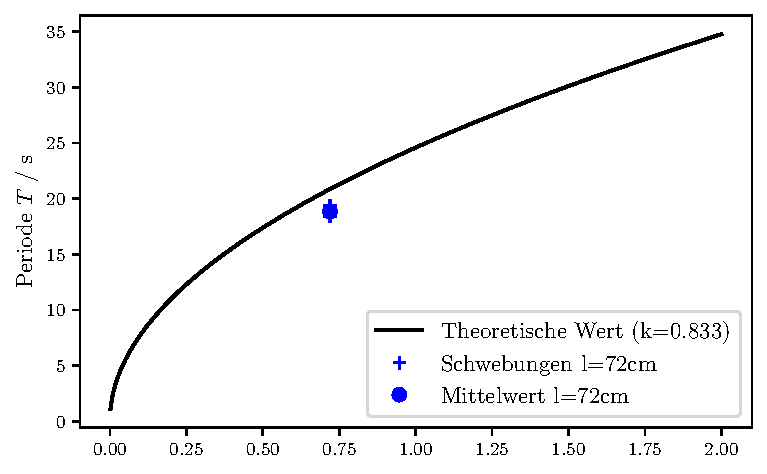
\includegraphics{build/plot8.pdf}
    \caption{Hall Spannung in Abhängigkeit vom Querstrom - Silber}
    \label{fig:Ag_I}
\end{figure}
Mit der Ausgleichsgeraden
\begin{align*}
    y &= mx + b\\
    m &= -0.0202\pm 0.0002\\
    b &=  0.0009\pm 0.0006\\
\end{align*}

\subsubsection{Hall Spannung bei konstantem Querstrom}
Um die Abhängigkeit der Hall Spannung vom äußeren Magnetfeld $B$ festzustellen wurde der Querstrom $I_q$ konstant auf 10 Ampere gehalten.
% Data 7
\begin{table}
    \centering
    \begin{tabular}{c c c}
        \toprule
        $I_{Spule} \;/\;$A & $U_H\;/\;$mV & $I_{durch} \;/\;$A\\
        \midrule
            0                   &-0,1707&             10\\
            0,5                 &-0,1740&             10\\
            1,0                 &-0,1777&             10\\
            1,5                 &-0,1809&             10\\
            2,0                 &-0,1850&             10\\
            2,5                 &-0,1885&             10\\
            3,0                 &-0,1909&             10\\
            3,5                 &-0,1945&             10\\
            4,0                 &-0,1970&             10\\
            4,5                 &-0,1990&             10\\
            5,0                 &-0,2002&             10\\
       \bottomrule
    \end{tabular}
    \caption{Hall Spannung für Silber- konstanter Durchflussstrom}
    \label{tab:Ag_I}
\end{table}
% Plot 7
\begin{figure}[H]
    \centering
    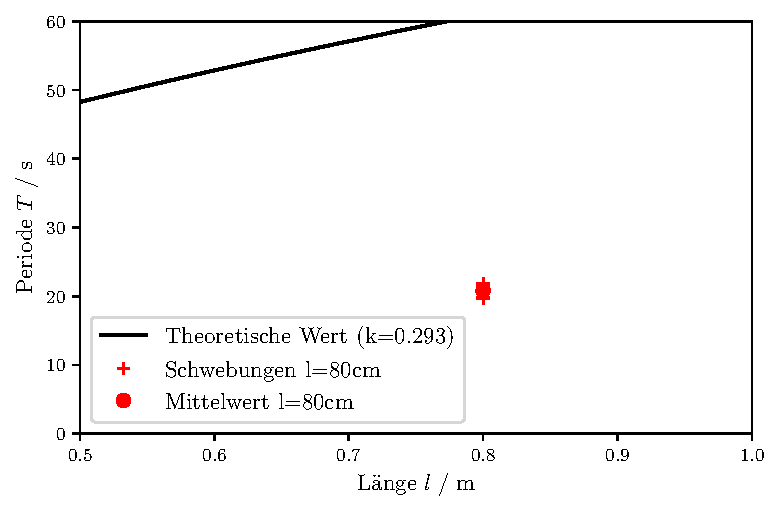
\includegraphics{build/plot7.pdf}
    \caption{Hall Spannung in Abhängigkeit vom Magnetfeld - Silber}
    \label{fig:Ag_B}
\end{figure}
Mit der Ausgleichsgeraden
\begin{align*}
    y &= mx + b\\
    m &= \cdot (-245 \pm 8)10^{-7}\\
    b &=  -0.1709\pm 0.0007 \\ % Signifikante Stellen????
\end{align*}

\subsubsection{Werte für die mikroskopischen Parameter}
%----------Tabelle
\begin{table}
    \centering
    \begin{tabular}{c c c c c}
        \toprule
        $U_H$ & $B$ & $n$  & $\bar{\tau}$ & $\vec{\bar{v}}_d$ \\
        \midrule
        $-0,1717\pm 0,0007$ & $33\pm 24          $          & $(1,0\pm 0,7)\cdot 10^{20}  $   & $(5\pm 4)\cdot 10^{-5}      $    & $16\pm 12 $ \\
        $-0,1748\pm 0,0007$ & $159\pm 24         $          & $(4,9\pm 0,7)\cdot 10^{20}  $   & $(1,14\pm 0,20)\cdot 10^{-5}$    & $79\pm 12 $ \\
        $-0,1779\pm 0,0007$ & $284\pm 25         $          & $(8,8\pm 0,8)\cdot 10^{20}  $   & $(6,3\pm 0,8)\cdot 10^{-6}  $    & $141\pm 12$  \\
        $-0,1810\pm 0,0008$ & $410\pm 26         $          & $(1,27\pm 0,08)\cdot 10^{21}$   & $(4,4\pm 0,5)\cdot 10^{-6}  $    & $204\pm 13$  \\
        $-0,1841\pm 0,0008$ & $535\pm 28         $          & $(1,66\pm 0,09)\cdot 10^{21}$   & $(3,4\pm 0,4)\cdot 10^{-6}  $    & $266\pm 14$  \\
        $-0,1871\pm 0,0009$ & $661\pm 31         $          & $(2,05\pm 0,10)\cdot 10^{21}$   & $(2,73\pm 0,28)\cdot 10^{-6}$    & $329\pm 15$  \\
        $-0,1902\pm 0,0010$ & $786\pm 33         $          & $(2,44\pm 0,11)\cdot 10^{21}$   & $(2,29\pm 0,23)\cdot 10^{-6}$    & $391\pm 17$  \\
        $-0,1933\pm 0,0011$ & $(9,1\pm 0,4)\cdot 10^{2}  $  & $(2,83\pm 0,11)\cdot 10^{21}$   & $(1,98\pm 0,20)\cdot 10^{-6}$    & $454\pm 18$  \\
        $-0,1964\pm 0,0012$ & $(1,04\pm 0,04)\cdot 10^{3}$  & $(3,22\pm 0,12)\cdot 10^{21}$   & $(1,74\pm 0,17)\cdot 10^{-6}$    & $516\pm 20$  \\
        $-0,1994\pm 0,0012$ & $(1,16\pm 0,04)\cdot 10^{3}$  & $(3,61\pm 0,13)\cdot 10^{21}$   & $(1,55\pm 0,15)\cdot 10^{-6}$    & $578\pm 22$  \\
        $-0,2025\pm 0,0013$ & $(1,29\pm 0,05)\cdot 10^{3}$  & $(4,00\pm 0,15)\cdot 10^{21}$   & $(1,40\pm 0,14)\cdot 10^{-6}$    & $641\pm 23$ \\
        \bottomrule
    \end{tabular}
    \caption{Parameter für Silber}
    \label{tab:Ag_B}
\end{table}

\begin{table}
    \centering
    \begin{tabular}{c c c c}
        \toprule
        $U_H$ & $|\bar{v}|$ & $\bar{l}$ & $\mu$ \\
        \midrule
        $-0,1717\pm 0,0007$  & $(1,7\pm 0,4)\cdot 10^{3}  $  & $0,09\pm 0,04    $  & $(2,1\pm 1,5)\cdot 10^{-7}$  \\
        $-0,1748\pm 0,0007$  & $(2,83\pm 0,14)\cdot 10^{3}$  & $0,032\pm 0,004  $  & $(1,00\pm 0,18)\cdot 10^{-6}$  \\
        $-0,1779\pm 0,0007$  & $(3,44\pm 0,10)\cdot 10^{3}$  & $0,0218\pm 0,0024$  & $(1,79\pm 0,23)\cdot 10^{-6}$  \\
        $-0,1810\pm 0,0008$  & $(3,88\pm 0,08)\cdot 10^{3}$  & $0,0171\pm 0,0017$  & $(2,58\pm 0,29)\cdot 10^{-6}$  \\
        $-0,1841\pm 0,0008$  & $(4,24\pm 0,08)\cdot 10^{3}$  & $0,0143\pm 0,0014$  & $(3,4\pm 0,4)\cdot 10^{-6}$  \\
        $-0,1871\pm 0,0009$  & $(4,55\pm 0,07)\cdot 10^{3}$  & $0,0124\pm 0,0012$  & $(4,2\pm 0,4)\cdot 10^{-6}$  \\
        $-0,1902\pm 0,0010$  & $(4,82\pm 0,07)\cdot 10^{3}$  & $0,0111\pm 0,0011$  & $(5,0\pm 0,5)\cdot 10^{-6}$  \\
        $-0,1933\pm 0,0011$  & $(5,07\pm 0,07)\cdot 10^{3}$  & $0,0100\pm 0,0010$  & $(5,7\pm 0,6)\cdot 10^{-6}$  \\
        $-0,1964\pm 0,0012$  & $(5,29\pm 0,07)\cdot 10^{3}$  & $0,0092\pm 0,0009$  & $(6,5\pm 0,7)\cdot 10^{-6}$  \\
        $-0,1994\pm 0,0012$  & $(5,49\pm 0,07)\cdot 10^{3}$  & $0,0085\pm 0,0008$  & $(7,3\pm 0,7)\cdot 10^{-6}$  \\
        $-0,2025\pm 0,0013$  & $(5,69\pm 0,07)\cdot 10^{3}$  & $0,0080\pm 0,0008$  & $(8,1\pm 0,8)\cdot 10^{-6}$ \\
        \bottomrule
    \end{tabular}
    \caption{Parameter 2 für Silber}
    \label{tab:Ag_B}
\end{table}


%|||||||||||||||||||||||||||||||||||||||||||||||||||||||||||||||||||||||||||||||||||||||||||||||||||||||||||||||||


% --------ZINK
\subsection{Zink}
\subsubsection{Geometrische Messungen und Wiederstand}
Für Zink geb es keine Probe um die geometrischen Werte zu  Messen, daher mussten die Werte recherchiert werden.
\begin{align*}
    \rho_{Zn,literatur} &= \SI{0,06}{\micro \ohm \meter} %https://oerttel.net/data/documents/Leitfaehigkeit.pdf
\end{align*}
\subsubsection{Hall Spannung bei konstantem B-Feld}
%Data 6
\begin{table}
    \centering
    \begin{tabular}{c c c}
        \toprule
        $I_{Spule} \;/\;$A & $U_H\;/\;$mV & $I_{durch} \;/\;$A\\
        \midrule
            5                   &-0,0012&             0\\
            5                   &-0,0373&             1\\
            5                   &-0,0755&             2\\
            5                   &-0,1136&             3\\
            5                   &-0,1530&             4\\
            5                   &-0,1919&             5\\
            5                   &-0,2291&             6\\
            5                   &-0,2671&             7\\
            5                   &-0,3090&             8\\
            5                   &-0,3512&             9\\
            5                   &-0,3957&             10\\
        \bottomrule
    \end{tabular}
    \caption{Hall Spannung für Zink- konstantes Magnetfeld}
    \label{tab:Zn_B}
\end{table}
%Plot 6
\begin{figure}[H]
    \centering
    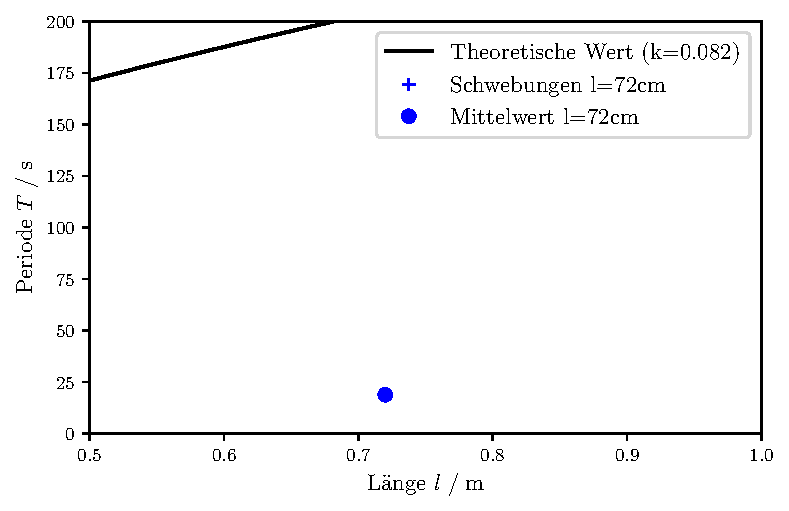
\includegraphics{build/plot6.pdf}
    \caption{Hall Spannung in Abhängigkeit vom Querstrom - Zink}
    \label{fig:Zn_B}
\end{figure}
Mit der Ausgleichsgeraden
\begin{align*}
    y &= mx + b\\
    m &= -0.03919\pm 0.00032\\
    b &=   0.0028\pm 0.0019\\ 
\end{align*}

\subsubsection{Hall Spannung bei konstantem Querstrom}
% Data 5
\begin{table}
    \centering
    \begin{tabular}{c c c}
        \toprule
        $I_{Spule} \;/\;$A & $U_H\;/\;$mV & $I_{durch} \;/\;$A\\
        \midrule
            0                   &-0,4094&             10\\
            0,5                 &-0,4042&             10\\
            1,0                 &-0,4024&             10\\
            1,5                 &-0,4004&             10\\
            2,0                 &-0,3981&             10\\
            2,5                 &-0,3981&             10\\
            3,0                 &-0,3950&             10\\
            3,5                 &-0,3928&             10\\
            4,0                 &-0,3900&             10\\
            4,5                 &-0,3880&             10\\
            5,0                 &-0,3800&             10\\
        \bottomrule
    \end{tabular}
    \caption{Hall Spannung für Zink- konstanter Durchflussstrom}
    \label{tab:Zn_B}
\end{table}
% Plot 5
\begin{figure}[H]
    \centering
    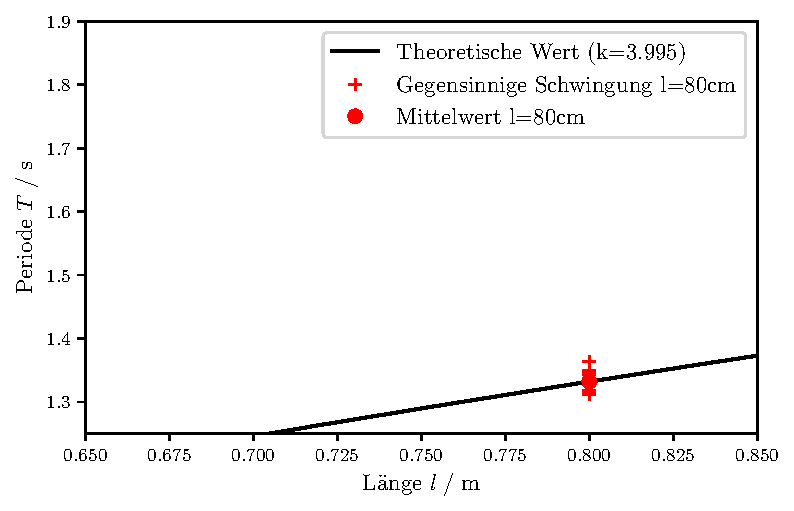
\includegraphics{build/plot5.pdf}
    \caption{Hall Spannung in Abhängigkeit vom Magnetfeld - Zink}
    \label{fig:Zn_B}
\end{figure}
Mit der Ausgleichsgeraden
\begin{align*}
    y &= mx + b\\
    m &= (1,93\pm 0,15)\cdot 10^{-5}\\
    b &=  -0.409006\pm 0.001123\\ % Signifikante Stellen????
\end{align*}

\subsubsection{Werte für die mikroskopischen Parameter}
%----------Tabelle
\begin{table}
    \centering
    \begin{tabular}{c c c c c}
        \toprule
        $U_H$ & $B$ & $n$  & $\bar{\tau}$ & $\vec{\bar{v}}_d$ \\
        \midrule
        $-0,4084\pm 0,0011$  & $33\pm 24          $              & $(5\pm 4)\cdot 10^{19}      $    & $(2,2\pm 1,6)\cdot 10^{-5}  $    & $8\pm 6    $   \\
        $-0,4059\pm 0,0011$  & $159\pm 24         $              & $(2,5\pm 0,4)\cdot 10^{20}  $    & $(4,7\pm 0,7)\cdot 10^{-6}  $    & $41\pm 6   $   \\
        $-0,4035\pm 0,0012$  & $284\pm 25         $              & $(4,6\pm 0,4)\cdot 10^{20}  $    & $(2,60\pm 0,23)\cdot 10^{-6}$    & $73\pm 6   $   \\
        $-0,4011\pm 0,0013$  & $410\pm 26         $              & $(6,6\pm 0,4)\cdot 10^{20}  $    & $(1,80\pm 0,12)\cdot 10^{-6}$    & $105\pm 7  $   \\
        $-0,3986\pm 0,0014$  & $535\pm 28         $              & $(8,6\pm 0,5)\cdot 10^{20}  $    & $(1,38\pm 0,07)\cdot 10^{-6}$    & $138\pm 7  $   \\
        $-0,3962\pm 0,0015$  & $661\pm 31         $              & $(1,06\pm 0,05)\cdot 10^{21}$    & $(1,12\pm 0,05)\cdot 10^{-6}$    & $170\pm 8  $   \\
        $-0,3938\pm 0,0016$  & $786\pm 33         $              & $(1,26\pm 0,05)\cdot 10^{21}$    & $(9,4\pm 0,4)\cdot 10^{-7}  $    & $202\pm 9  $   \\
        $-0,3914\pm 0,0017$  & $(9,1\pm 0,4)\cdot 10^{02}  $     & $(1,46\pm 0,06)\cdot 10^{21}$    & $(8,09\pm 0,33)\cdot 10^{-7}$    & $234\pm 10 $   \\
        $-0,3889\pm 0,0019$  & $(1,04\pm 0,04)\cdot 10^{03}$     & $(1,66\pm 0,07)\cdot 10^{21}$    & $(7,11\pm 0,28)\cdot 10^{-7}$    & $267\pm 10 $   \\
        $-0,3865\pm 0,0020$  & $(1,16\pm 0,04)\cdot 10^{03}$     & $(1,87\pm 0,07)\cdot 10^{21}$    & $(6,34\pm 0,24)\cdot 10^{-7}$    & $299\pm 11 $   \\
        $-0,3841\pm 0,0022$  & $(1,29\pm 0,05)\cdot 10^{03}$     & $(2,07\pm 0,08)\cdot 10^{21}$    & $(5,72\pm 0,21)\cdot 10^{-7}$    & $331\pm 12 $   \\
        \bottomrule
    \end{tabular}
    \caption{Parameter für Zink}
    \label{tab:Ag_B}
\end{table}

\begin{table}
    \centering
    \begin{tabular}{c c c c}
        \toprule
        $U_H$ & $|\bar{v}|$ & $\bar{l}$ & $\mu$ \\
        \midrule
        $-0,4084\pm 0,0011$  & $(1,34\pm 0,32)\cdot 10^{3}$  & $0,030\pm 0,014    $  & $(5\pm 4)\cdot 10^{-7}      $   \\
        $-0,4059\pm 0,0011$  & $(2,27\pm 0,11)\cdot 10^{3}$  & $0,0106\pm 0,0011  $  & $(2,4\pm 0,4)\cdot 10^{-6}  $   \\
        $-0,4035\pm 0,0012$  & $(2,76\pm 0,08)\cdot 10^{3}$  & $0,0072\pm 0,0004  $  & $(4,4\pm 0,4)\cdot 10^{-6}  $   \\
        $-0,4011\pm 0,0013$  & $(3,11\pm 0,07)\cdot 10^{3}$  & $0,00561\pm 0,00024$  & $(6,3\pm 0,4)\cdot 10^{-6}  $   \\
        $-0,3986\pm 0,0014$  & $(3,40\pm 0,06)\cdot 10^{3}$  & $0,00469\pm 0,00017$  & $(8,3\pm 0,4)\cdot 10^{-6}  $   \\
        $-0,3962\pm 0,0015$  & $(3,65\pm 0,06)\cdot 10^{3}$  & $0,00408\pm 0,00013$  & $(1,02\pm 0,05)\cdot 10^{-5}$   \\
        $-0,3938\pm 0,0016$  & $(3,87\pm 0,06)\cdot 10^{3}$  & $0,00363\pm 0,00011$  & $(1,21\pm 0,05)\cdot 10^{-5}$   \\
        $-0,3914\pm 0,0017$  & $(4,07\pm 0,06)\cdot 10^{3}$  & $0,00329\pm 0,00009$  & $(1,41\pm 0,06)\cdot 10^{-5}$   \\
        $-0,3889\pm 0,0019$  & $(4,24\pm 0,06)\cdot 10^{3}$  & $0,00302\pm 0,00008$  & $(1,60\pm 0,06)\cdot 10^{-5}$   \\
        $-0,3865\pm 0,0020$  & $(4,41\pm 0,06)\cdot 10^{3}$  & $0,00280\pm 0,00007$  & $(1,79\pm 0,07)\cdot 10^{-5}$   \\
        $-0,3841\pm 0,0022$  & $(4,56\pm 0,06)\cdot 10^{3}$  & $0,00261\pm 0,00006$  & $(1,99\pm 0,07)\cdot 10^{-5}$   \\
        \bottomrule
    \end{tabular}
    \caption{Parameter 2 für Zink}
    \label{tab:Ag_B}
\end{table}

\label{sec:Auswertung}
